\chapter{Seismic Network}
\label{chap:quakeNetwork}
In this chapter we explain how the seismic network is constructed, based on all the data processed from the seismic database into our earthquakes table and we show two methods of analyzing this network and the results obtained, mainly the scale-free nature of these characteristics through suggestive visualizations.


%---------------------------------------------------------------
\section{How to construct a Seismic Network}
\label{subsection:seismicNetwork}
After splitting the region into cubes and assigning each earthquake into it's respective cube we can begin building our network. Similar to \cite{Abe_2004}, this is done by iterating chronologically through the earthquakes table as follows:
\begin{enumerate}
	\item When you encounter an event create a node with the label $cubeIndex$ defined earlier in our table. Our graph nodes represent the cubes that we split our region in, so when we say cube/node we refer to the same thing.
	\item Pick the next event chronologically and create a node for it.
	\item Now we have two options, to consider edge weights\footnotemark or not:
	\begin{itemize}
		\item If we consider edge weights, first check if there is already an edge between the two nodes that we placed. If there is, add $1$ to the weight of this edge; if there isn't, create the edge.
		\item If we don't consider edge weights, simply create the edge between the nodes; if there is already an edge, creating a new one on top of the old changes nothing, at the end the edge still counts as a single one.
	\end{itemize}
	\item Two nodes may sometimes coincide with each other (succesive events in the same cube), forming a loop.
	\item Repeat from step 2.
	\item At the end, after the network is complete, for each node we can add different attributes based on the task we wish to perform on the graph. We can add the cube coordinates (x, y, z) or the real cube coordinates (cubeLatitude, cubeLongitude, cubeDepth). Also we can add the list of all the events that occured in that specific cube.
	
	
\footnotetext{Considering edge weights ultimately changes the connectivity distribution of the network (because certain nodes degrees will increase when taking into account the weight) so it is useful to study the network from both perspectives.}

\end{enumerate}

\begin{figure}
\centering
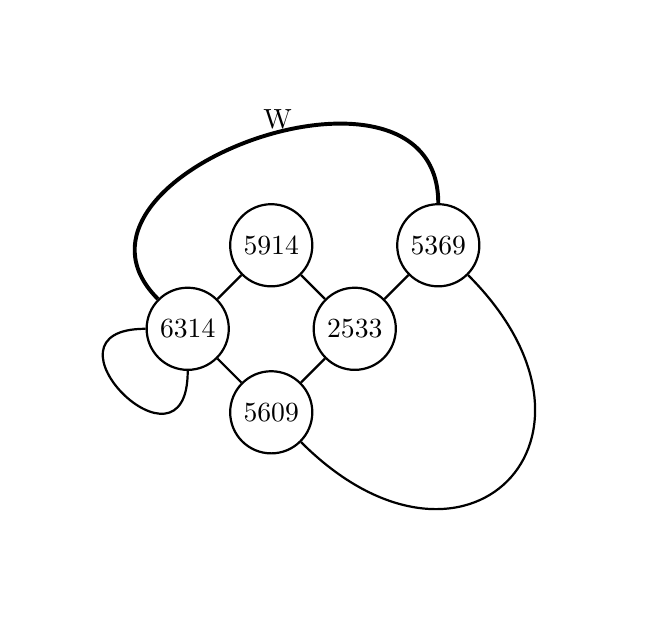
\begin{tikzpicture}[node distance={15mm}, thick, main/.style = {draw, circle}] 
\node[main] (1) {$6314$}; 
\node[main] (2) [above right of=1] {$5914$}; 
\node[main] (3) [below right of=1] {$5609$}; 
\node[main] (4) [above right of=3] {$2533$}; 
\node[main] (5) [above right of=4] {$5369$}; 

\draw(1) -- (2); 
\draw(1) -- (3); 
\draw [line width=0.05cm] (1) to [out=135,in=90,looseness=1.5] node[midway, above right] {W}  (5); 
\draw (1) to [out=180,in=270,looseness=5] (1); 
\draw (2) -- (4); 
\draw (3) -- (4); 
\draw (5) -- (4); 
\draw (5) to [out=315, in=315, looseness=2.5]  (3); 

\end{tikzpicture} 
\caption{Seismic Network (Graph representation) example: Nodes are identified as $cubeIndex$. This indexing makes it easy to acces any information about events in that respective cube from our Earthquakes Table. Also, if the network is weighted, this can be represented on the edge as $W$, where each additional link between two nodes increases this value by 1.}
\end{figure}

So now we posses the two fundamental tools used in our following analysis, the earthquakes table and the seismic network


%---------------------------------------------------------------
\section{Centrality Measures of a Network}
The fundamental measure to describe our seismic network is the connectivity distribution $P(k)$ \cite{latora}. This distribution comes naturally by realising the histogram of the nodes degree and computing the distribution. We also fit the log-log plot of this distribution and show that it is scale-free.

\begin{equation}
P(k) \sim k^{-\gamma}
\end{equation}

The connectivity computations are made for various seismic networks (Vrancea(Romania), California(USA), Italy and Japan), with different magnitude restrictions, for 2 cube sizes: $5\times5\times5$ km and $10\times10\times10$ km, with and without edge weights.

% ---------------------------- VRANCEA CONNECTIVITY ----------------------------%
\clearpage
\paragraph{Vrancea} - Connectivity
\begin{figure}[!h]
\begin{subfigure}{.99\textwidth}
  \centering
  \includegraphics[width=.85\columnwidth]{connectivityVrancea_1magnitude10}
  \caption{$1 \leq magnitude$}
  \label{fig:conVr1mag10}
\end{subfigure}%

\begin{subfigure}{.99\textwidth}
  \centering
  \includegraphics[width=.85\columnwidth]{connectivityVrancea_2magnitude10}
  \caption{$2 \leq magnitude$}
  \label{fig:conVr2mag10}
\end{subfigure}%

\begin{subfigure}{.99\textwidth}
  \centering
  \includegraphics[width=.85\columnwidth]{connectivityVrancea_2magnitude4}
  \caption{$2\leq magnitude \leq 4$}
  \label{fig:conVr2mag14}
\end{subfigure}%

\begin{subfigure}{.99\textwidth}
  \centering
  \includegraphics[width=.85\columnwidth]{connectivityVrancea_3magnitude7}
  \caption{$3 \leq magnitude \leq 7$}
  \label{fig:conVr3mag7}
\end{subfigure}%

\caption{Connectivity distribution $P(k)$ for Vrancea in log-log and linear interpolation of the results, for a number of magnitude ranges. For each range, two granularization sizes of the seismic areas have been chosen: on the left $5 \times 5 \times5 $ km cubes and on the right $10 \times 10 \times 10$ km cubes. The exponent of the fit, $\gamma$ ranges from $\sim 1.08$ to $1.756$.}
\label{fig:connectivityVr}
\end{figure}

\clearpage
\paragraph{Vrancea} - Connectivity Weighted
\begin{figure}[!h]
\begin{subfigure}{.99\textwidth}
  \centering
  \includegraphics[width=.85\columnwidth]{connectivityVranceaWeighted_1magnitude10}
  \caption{$1 \leq magnitude$}
  \label{fig:conWeiVr1mag10}
\end{subfigure}%

\begin{subfigure}{.99\textwidth}
  \centering
  \includegraphics[width=.85\columnwidth]{connectivityVranceaWeighted_2magnitude10}
  \caption{$2 \leq magnitude$}
  \label{fig:conWeiVr2mag10}
\end{subfigure}%

\begin{subfigure}{.99\textwidth}
  \centering
  \includegraphics[width=.85\columnwidth]{connectivityVranceaWeighted_2magnitude4}
  \caption{$2\leq magnitude \leq 4$}
  \label{fig:conWeiVr2mag4}
\end{subfigure}%

\begin{subfigure}{.99\textwidth}
  \centering
  \includegraphics[width=.85\columnwidth]{connectivityVranceaWeighted_3magnitude7}
  \caption{$3 \leq magnitude \leq 7$}
  \label{fig:conWeiVr3mag7}
\end{subfigure}%

\caption{Weighted connectivity distribution $P(k)$ for Vrancea in log-log and linear interpolation of the results, for a number of magnitude ranges. For each range, two granularization sizes of the seismic areas have been chosen: on the left $5 \times 5 \times5 $ km cubes and on the right $10 \times 10 \times 10$ km cubes. The exponent of the fit, $\gamma$ ranges from $\sim 1.95$ to $3.26$.}
\label{fig:connectivityVrWeighted}
\end{figure}


% ---------------------------- California CONNECTIVITY ----------------------------%
\clearpage
\paragraph{California} - Connectivity
\begin{figure}[!h]
\begin{subfigure}{.99\textwidth}
  \centering
  \includegraphics[width=.85\columnwidth]{connectivityCalifornia_1magnitude10}
  \caption{$1 \leq magnitude$}
  \label{fig:conCa1mag10}
\end{subfigure}%

\begin{subfigure}{.99\textwidth}
  \centering
  \includegraphics[width=.85\columnwidth]{connectivityCalifornia_2magnitude10}
  \caption{$2\leq magnitude$}
  \label{fig:conCa2mag10}
\end{subfigure}%

\begin{subfigure}{.99\textwidth}
  \centering
  \includegraphics[width=.85\columnwidth]{connectivityCalifornia_1magnitude3}
  \caption{$1 \leq magnitude \leq 3$}
  \label{fig:conCa1mag3}
\end{subfigure}%

\begin{subfigure}{.99\textwidth}
  \centering
  \includegraphics[width=.85\columnwidth]{connectivityCalifornia_2magnitude4}
  \caption{$2 \leq magnitude \leq 4$}
  \label{fig:conCa2mag4}
\end{subfigure}%

\caption{Connectivity distribution $P(k)$ for California in log-log and linear interpolation of the results, for a number of magnitude ranges. For each range, two granularization sizes of the seismic areas have been chosen: on the left $5 \times 5 \times5 $ km cubes and on the right $10 \times 10 \times 10$ km cubes. The exponent of the fit, $\gamma$ ranges from $\sim 1.45$ to $2.16$.}
\label{fig:connectivityCa}
\end{figure}

\clearpage
\paragraph{California} - Connectivity Weighted
\begin{figure}[!h]
\begin{subfigure}{.99\textwidth}
  \centering
  \includegraphics[width=.85\columnwidth]{connectivityCaliforniaWeighted_1magnitude10}
  \caption{$1 \leq magnitude$}
  \label{fig:conWeiCa1mag10}
\end{subfigure}%

\begin{subfigure}{.99\textwidth}
  \centering
  \includegraphics[width=.85\columnwidth]{connectivityCaliforniaWeighted_2magnitude10}
  \caption{$2\leq magnitude$}
  \label{fig:conWeiCa2mag10}
\end{subfigure}%

\begin{subfigure}{.99\textwidth}
  \centering
  \includegraphics[width=.85\columnwidth]{connectivityCaliforniaWeighted_1magnitude3}
  \caption{$1 \leq magnitude \leq 3$}
  \label{fig:conWeiCa1mag3}
\end{subfigure}%

\begin{subfigure}{.99\textwidth}
  \centering
  \includegraphics[width=.85\columnwidth]{connectivityCaliforniaWeighted_2magnitude4}
  \caption{$2 \leq magnitude \leq 4$}
  \label{fig:conWeiCa2mag4}
\end{subfigure}%


\caption{Weighted connectivity distribution $P(k)$ for California in log-log and linear interpolation of the results, for a number of magnitude ranges. For each range, two granularization sizes of the seismic areas have been chosen: on the left $5 \times 5 \times5 $ km cubes and on the right $10 \times 10 \times 10$ km cubes. The exponent of the fit, $\gamma$ ranges from $\sim 2.06$ to $2.71$.}
\label{fig:connectivityCaWeighted}
\end{figure}


% ---------------------------- Italy CONNECTIVITY ----------------------------%
\clearpage
\paragraph{Italy} - Connectivity
\begin{figure}[!h]
\begin{subfigure}{.99\textwidth}
  \centering
  \includegraphics[width=.85\columnwidth]{connectivityItaly_1magnitude10}
  \caption{$1 \leq magnitude$}
  \label{fig:conIt1mag10}
\end{subfigure}%

\begin{subfigure}{.99\textwidth}
  \centering
  \includegraphics[width=.85\columnwidth]{connectivityItaly_2magnitude10}
  \caption{$2\leq magnitude$}
  \label{fig:conIt2mag10}
\end{subfigure}%

\begin{subfigure}{.99\textwidth}
  \centering
  \includegraphics[width=.85\columnwidth]{connectivityItaly_1magnitude3}
  \caption{$1 \leq magnitude \leq 3$}
  \label{fig:conIt1mag3}
\end{subfigure}%

\begin{subfigure}{.99\textwidth}
  \centering
  \includegraphics[width=.85\columnwidth]{connectivityItaly_2magnitude4}
  \caption{$2 \leq magnitude \leq 4$}
  \label{fig:conIt2mag4}
\end{subfigure}%

\caption{Connectivity distribution $P(k)$ for Italy in log-log and linear interpolation of the results, for a number of magnitude ranges. For each range, two granularization sizes of the seismic areas have been chosen: on the left $5 \times 5 \times5 $ km cubes and on the right $10 \times 10 \times 10$ km cubes. The exponent of the fit, $\gamma$ ranges from $\sim 1.44$ to $2.3$.}
\label{fig:connectivityIt}
\end{figure}

\clearpage
\paragraph{Italy} - Connectivity Weighted
\begin{figure}[!h]
\begin{subfigure}{.99\textwidth}
  \centering
  \includegraphics[width=.85\columnwidth]{connectivityItalyWeighted_1magnitude10}
  \caption{$1 \leq magnitude$}
  \label{fig:conWeiIt1mag10}
\end{subfigure}%

\begin{subfigure}{.99\textwidth}
  \centering
  \includegraphics[width=.85\columnwidth]{connectivityItalyWeighted_2magnitude10}
  \caption{$1 \leq magnitude$}
  \label{fig:conWeiIt2mag10}
\end{subfigure}%

\begin{subfigure}{.99\textwidth}
  \centering
  \includegraphics[width=.85\columnwidth]{connectivityItalyWeighted_1magnitude3}
  \caption{$1 \leq magnitude \leq 3$}
  \label{fig:conWeiIt1mag3}
\end{subfigure}%

\begin{subfigure}{.99\textwidth}
  \centering
  \includegraphics[width=.85\columnwidth]{connectivityItalyWeighted_2magnitude4}
  \caption{$2 \leq magnitude \leq 4$}
  \label{fig:conWeiIt2mag4}
\end{subfigure}%

\caption{Weighted connectivity distribution $P(k)$ for Italy in log-log and linear interpolation of the results, for a number of magnitude ranges. For each range, two granularization sizes of the seismic areas have been chosen: on the left $5 \times 5 \times5 $ km cubes and on the right $10 \times 10 \times 10$ km cubes. The exponent of the fit, $\gamma$ ranges from $\sim 2.8$ to $3.72$.}
\label{fig:connectivityItWeighted}
\end{figure}


% ---------------------------- Japan CONNECTIVITY ----------------------------%
\clearpage
\paragraph{Japan} - Connectivity
\begin{figure}[!h]
\begin{subfigure}{.99\textwidth}
  \centering
  \includegraphics[width=.85\columnwidth]{connectivityJapan_1magnitude10}
  \caption{$1 \leq magnitude$}
  \label{fig:conJa1mag10}
\end{subfigure}%

\begin{subfigure}{.99\textwidth}
  \centering
  \includegraphics[width=.85\columnwidth]{connectivityJapan_2magnitude10}
  \caption{$2\leq magnitude$}
  \label{fig:conJa2mag10}
\end{subfigure}%

\begin{subfigure}{.99\textwidth}
  \centering
  \includegraphics[width=.85\columnwidth]{connectivityJapan_1magnitude3}
  \caption{$1 \leq magnitude \leq 3$}
  \label{fig:conJa1mag3}
\end{subfigure}%

\begin{subfigure}{.99\textwidth}
  \centering
  \includegraphics[width=.85\columnwidth]{connectivityJapan_2magnitude4}
  \caption{$2 \leq magnitude \leq 4$}
  \label{fig:conJa2mag4}
\end{subfigure}%

\caption{Connectivity distribution $P(k)$ for Japan in log-log and linear interpolation of the results, for a number of magnitude ranges. For each range, two granularization sizes of the seismic areas have been chosen: on the left $5 \times 5 \times5 $ km cubes and on the right $10 \times 10 \times 10$ km cubes. The exponent of the fit, $\gamma$ ranges from $\sim 1.87$ to $2.5$.}
\label{fig:connectivityJa}
\end{figure}

\clearpage
\paragraph{Japan} - Connectivity Weighted
\begin{figure}[!h]
\begin{subfigure}{.99\textwidth}
  \centering
  \includegraphics[width=.85\columnwidth]{connectivityJapanWeighted_1magnitude10}
  \caption{$1 \leq magnitude$}
  \label{fig:conWeiJa1mag10}
\end{subfigure}%

\begin{subfigure}{.99\textwidth}
  \centering
  \includegraphics[width=.85\columnwidth]{connectivityJapanWeighted_2magnitude10}
  \caption{$2\leq magnitude$}
  \label{fig:conWeiJa2mag10}
\end{subfigure}%

\begin{subfigure}{.99\textwidth}
  \centering
  \includegraphics[width=.85\columnwidth]{connectivityJapanWeighted_1magnitude3}
  \caption{$1\leq magnitude \leq 3$}
  \label{fig:conWeiJa1mag3}
\end{subfigure}%

\begin{subfigure}{.99\textwidth}
  \centering
  \includegraphics[width=.85\columnwidth]{connectivityJapanWeighted_2magnitude4}
  \caption{$2 \leq magnitude \leq 4$}
  \label{fig:conWeiJa2mag4}
\end{subfigure}%

\caption{Weighted connectivity distribution $P(k)$ for Japan in log-log and linear interpolation of the results, for a number of magnitude ranges. For each range, two granularization sizes of the seismic areas have been chosen: on the left $5 \times 5 \times5 $ km cubes and on the right $10 \times 10 \times 10$ km cubes. The exponent of the fit, $\gamma$ ranges from $\sim 2.45$ to $3.17$.}
\label{fig:connectivityItWeighted}
\end{figure}


\clearpage
%---------------------------------------------------------------
\section{Network Cycles and Motifs}
In this section the general approach to define and detect the building blocks of a network is being described \cite{latora}.\par 
In social and biological networks it has been noticed that triangles are highly recurrent, so work has been done in identifying where and why these kind of patterns appear. They are generally called {\it cycles} of different lengths $C_l$ and other subgraphs known as {\it motifs} $F_{n,l}$, which represent cycles that occur in {\it real networks} more frequently than in their corresponding random counterparts.


%----------%--------------%---------------------------------
\subsection{Motifs}
Network motifs are sub-graphs that repeat themselves in a specific network or even among various networks. Each of these sub-graphs, defined by a particular pattern of interactions between vertices, may reflect a framework in which particular functions are achieved efficiently. They have gathered much attention as a useful concept to uncover structural and functional design principles of complex networks. In bioinformatics, network motifs have been applied to various applications including prediction of protein interactions, identifying breast cancer related genes, and detection of essential proteins. Although network motifs may provide a deep insight into the network's functional abilities, their detection is computationally challenging.\par 

Given an undirected graph $G=(\mathcal{N},\mathcal{L})$ and any possible small connected graph $F_{n,l}$ with $n$ nodes and $l$ links, we wish to find out if $F$ is a significant subgraph of $G$. This is done by comparing the number of subgraphs of $G$ isomorphic to $F$ with the number of subraphs of a randomised network $G'=(\mathcal{N},\mathcal{L})$ isomorphic to $F$.\\
The simplest approach to quantify the relevance of $F_{n,l}$ as a subgraph of $G$ is based on the evaluation of the {\it Z-score}, defined as follows:
\begin{equation}
Z_F = \frac{n_f - \bar{n}^{rand}_F}{\sigma_{n_F}^{rand}}
\end{equation}
where $n_F$ is the number of times the subgraph $F_{n,l}$ appears in $G$ and $\bar{n}^{rand}_F$ and $\sigma_{n_F}^{rand}$ are the mean and the standard deviation, respectively, of the number of occurences in an ensemble of graphs obtained by randomising $G$.\par 
The absolute value of $Z_F$ indicates the distance between observed number of occurences and expected number of occurences in a corresponding ensemble of randomized networks with $N$ and $K$ equal to those of our network $G$, in units of standard deviations. We are interested in values of $Z_F$ larger than 2, meaning that the number of occurences is two standard deviations larger than $\bar{n}^{rand}_F$, which is a good indicator that the observed number of occurences are due to fluctuations only in $2.14\%$. Even better, when $Z_F=3$, the percentage drops to $0.13\%$, so a very good indication that $F_{n,l}$ is a network motif.


%----------%--------------%---------------------------------
\subsection{Motifs detection using NemoSuite}
NemoSuite \cite{nemosuite} (Network Motif Analysis in a Suite) is a web program developed and hosted online by researchers at University of Washington Bothell CSSE to detect and analyze network motifs. A network motif is a frequent and unique subgraph pattern in an input network, and it is determined by P-value beings smaller than 0.05 or Z-score being larger than 2.\par 

Network motif detection methods can be categorized into {\it network-centric} and {\it motif-centric} methods:
\begin{itemize}
	\item {\bf Nemo}: {\it Network-centric} approach searches all possible non-isomorphic subgraph patterns with a size (typically 3 to 8) and determines a pattern as a motif if the frequency of it is relatively high compared in a corresponding random graph. The network-centric motif detection program improves an ESU (Enumerate SUbgraphs) algorithm introduced by Sebastian Wernicke \cite{ESUmotifs} and has more functionality and output formats (NemoCount, NemoProfile, and NemoCollect). We are interested in these for the instance collection capability.
	
	\item {\bf NemoMapPy}: {\it Motif-centric} approach determines whether the given subgraph pattern is network motif by providing its frequency in an input network. Motif-centric method can determine large size of network motifs (typically larger than 8) by focusing on searching the given pattern. The program implements the NemoMap \cite{nemomap} algorithm developed by the same group and ported to python, which is based on Grochow and Kellis algorithm \cite{GK} and MODA program \cite{MODA}.
\end{itemize}


After creating the seismic network as described in \ref{subsection:seismicNetwork}, for different magnitude restrictions, we used the NemoSuite web application to identify and collect the 3 and 4 nodes motifs (triangles and tetrahedrons) in the network.\par
 Having the motif nodes, our goal is to plot the distribution of the surfaces (for the 3 nodes motifs) and volumes (for the 4 nodes motifs) weighted by the mean and total energy released by the earthquakes in the cubes that form each motif.

\clearpage
%----------%--------------%---------------------------------
\subsection{Triangle Surfaces}
For the 3 nodes motifs, calculations proceeds as follows:
\begin{itemize}

	\item Firstly we need to calculate the mean energy in each motif. The NemoSuite application \cite{nemosuite} extracts the node names of each motif from our network and using the "earthquakes list" attribute of each node we can identify every earthquake in each motif. Using the earthquakes table we can compute the {\it total energy} release of the earthquakes in each triangle, and by dividing by the total number of earthquakes in the motif we obtain the {\it mean energy} released.
	
	\item Then we use the motif nodes to calculate the surface of each motif. By having the geographical coordinates of each node, we use python's geopy library to calculate the exact "flat" distance along geodesic between two points using latitude and longitude in kilometers, and then we use pythagorean theorem to calculate the distance between the points, including the depth. Example for two points $X(lat,long,depth)$ and $Y(lat2,long2,depth2)$, $XY$ being the side of the respectie triangle:
	\begin{equation}
	\begin{split}
	&flatDistance = distance(X(lat,long),Y(lat2,long2)).km,\\
	&distance().km = \text{geopy distance function in km},\\
	&XY = \sqrt{flatDistance^2 +(X(depth)-Y(depth2))^2.}
	\end{split}
	\end{equation}
	
	\item After calculating all 3 sides of the triangle, we use Heron's formula for triangle surface:
	\begin{equation}
	\begin{split}
	&S = \sqrt{sp*(sp-a)*(sp-b)*(sp-c)},  \\
	&sp = \frac{a+b+c}{2}, \\
	&a,b,c = \text{the sides of the triangle}.
	\end{split}
	\end{equation}	
	
	\item We use the mean and total energy release per motif and the motif's surface to calculate the distribution of motifs surfaces weighted by mean or total energy.
	
	\item Compute the regression of the distribution in log-log space.
\end{itemize}

The computations are made for various seismic networks (Vrancea(Romania), California(USA) and Italy), with different magnitude restrictions, for 2 cube sizes: $5\times5\times5$ km and $10\times10\times10$ km.

% ---------------------- VRANCEA TRIANGLES -------------------

\clearpage
\paragraph{Vrancea} Mean Energy Weighted Surfaces
\begin{figure}[h!]
\begin{subfigure}{.99\textwidth}
  \centering
  \includegraphics[width=.85\columnwidth]{quakesVrancea_meanEnergy_1mag_trianglesAreas}
  \caption{$1 \leq magnitude$}
  \label{fig:trianglesVrME1}
\end{subfigure}%

\begin{subfigure}{.99\textwidth}
  \centering
  \includegraphics[width=.85\columnwidth]{quakesVrancea_meanEnergy_2mag_trianglesAreas}
  \caption{$2 \leq magnitude$}
  \label{fig:trianglesVrME2}
\end{subfigure}%

\begin{subfigure}{.99\textwidth}
  \centering
  \includegraphics[width=.85\columnwidth]{quakesVrancea_meanEnergy_3mag_trianglesAreas}
  \caption{$3 \leq magnitude$}
  \label{fig:trianglesVrME3}
\end{subfigure}%

\caption{$S_{ME} = Surface/Mean$ $Energy$ distribution in log-log plots for triangle motifs in Vrancea for 3 magnitude restrictions. The resulting interpolation shows that the distribution appears scale-free with $\gamma$ ranging from $\sim 1.14$ to $2.1$ }
\label{fig:trianglesSurfacesVrME}
\end{figure}


\clearpage
\paragraph{Vrancea} - Total Energy Weighted Surfaces
\begin{figure}[h!]

\begin{subfigure}{.99\textwidth}
  \centering
  \includegraphics[width=.85\columnwidth]{quakesVrancea_totalEnergy_1mag_trianglesAreas}
  \caption{$1 \leq magnitude$}
  \label{fig:trianglesVrTE1}
\end{subfigure}%

\begin{subfigure}{.99\textwidth}
  \centering
  \includegraphics[width=.85\columnwidth]{quakesVrancea_totalEnergy_2mag_trianglesAreas}
  \caption{$2 \leq magnitude$}
  \label{fig:trianglesVrTE2}
\end{subfigure}%

\begin{subfigure}{.99\textwidth}
  \centering
  \includegraphics[width=.85\columnwidth]{quakesVrancea_totalEnergy_3mag_trianglesAreas}
  \caption{$3 \leq magnitude$}
  \label{fig:trianglesVrTe3}
\end{subfigure}%

\caption{$S_{TE} = Surface/Total$ $Energy$ distribution in log-log plots for triangle motifs in Vrancea for 3 magnitude restrictions. The resulting interpolation shows that the distribution appears scale-free with $\gamma$ ranging from $\sim 2.79$ to $3.67$ }
\label{fig:trianglesSurfacesVrTE}
\end{figure}


\clearpage
% ---------------------- CALIFORNIA TRIANGLES -------------------____%
\paragraph{California} - Mean Energy Weighted Surfaces
\begin{figure}[h!]

\begin{subfigure}{.99\textwidth}
  \centering
  \includegraphics[width=.85\columnwidth]{quakesCalifornia_meanEnergy_2mag_trianglesAreas}
  \caption{$2 \leq magnitude$}
  \label{fig:trianglesCaME2}
\end{subfigure}%

\begin{subfigure}{.99\textwidth}
  \centering
  \includegraphics[width=.85\columnwidth]{quakesCalifornia_meanEnergy_3mag_trianglesAreas}
  \caption{$3 \leq magnitude$}
  \label{fig:trianglesCaME3}
\end{subfigure}%

\caption{$S_{ME} = Surface/Mean$ $Energy$ distribution in log-log plots for triangle motifs in California for 2 magnitude restrictions. The resulting interpolation shows that the distribution appears scale-free with $\gamma$ ranging from $\sim 1.42$ to $4.46$}
\label{fig:trianglesSurfacesCaME}
\end{figure}


\clearpage
\paragraph{California} - Total Energy Weighted Surfaces
\begin{figure}[h!]

\begin{subfigure}{.99\textwidth}
  \centering
  \includegraphics[width=.85\columnwidth]{quakesCalifornia_totalEnergy_2mag_trianglesAreas}
  \caption{$2 \leq magnitude$}
  \label{fig:trianglesCaTE2}
\end{subfigure}%

\begin{subfigure}{.99\textwidth}
  \centering
  \includegraphics[width=.85\columnwidth]{quakesCalifornia_totalEnergy_3mag_trianglesAreas}
  \caption{$3 \leq magnitude$}
  \label{fig:trianglesCaTe3}
\end{subfigure}%

\caption{$S_{TE} = Surface/Total$ $Energy$ distribution in log-log plots for triangle motifs in California for 2 magnitude restrictions. The resulting interpolation shows that the distribution appears scale-free with $\gamma$ ranging from $\sim 2.56$ to $5.01$ }
\label{fig:trianglesSurfacesCaTE}
\end{figure}


\clearpage
% ---------------------- Italy TRIANGLES -------------------____%
\paragraph{Italy} - Mean Energy Weighted Surfaces
\begin{figure}[h!]

%\begin{subfigure}{.99\textwidth}
  \centering
  \includegraphics[width=.85\columnwidth]{quakesItaly_meanEnergy_2mag_trianglesAreas}
  \caption{$2 \leq magnitude$}
  \label{fig:trianglesItME2}
%\end{subfigure}%

%\begin{subfigure}{.99\textwidth}
%  \centering
%  \includegraphics[width=.85\columnwidth]{quakesItaly_meanEnergy_3mag_trianglesAreas}
%  \caption{$3 \leq magnitude$}
%  \label{fig:trianglesItME3}
%\end{subfigure}%

\caption{$S_{ME} = Surface/Mean$ $Energy$ distribution in log-log plots for triangle motifs in Italy for $2 \leq magnitude$. The resulting interpolation shows that the distribution appears scale-free better at 10 km cube side granularization, with $\gamma = 1.503$ }
\label{fig:trianglesSurfacesItME}
\end{figure}


\paragraph{Italy} - Total Energy Weighted Surfaces
\begin{figure}[h!]

%\begin{subfigure}{.99\textwidth}
  \centering
  \includegraphics[width=.85\columnwidth]{quakesItaly_totalEnergy_2mag_trianglesAreas}
%  \caption{$2 \leq magnitude$}
  \label{fig:trianglesItTE2}
%\end{subfigure}%

%\begin{subfigure}{.99\textwidth}
%  \centering
%  \includegraphics[width=.85\columnwidth]{quakesItaly_totalEnergy_3mag_trianglesAreas}
%  \caption{$3 \leq magnitude$}
%  \label{fig:trianglesItTe3}
%\end{subfigure}%

\caption{$S_{TE} = Surface/Total$ $Energy$ distribution in log-log plots for triangle motifs in Italy for $2 \leq magnitude$. The resulting interpolation shows that the distribution appears scale-free better at 10 km cube side granularization, with $\gamma = 3.44$}
\label{fig:trianglesSurfacesItTE}
\end{figure}

\clearpage
%----------%--------------%---------------------------------
\subsection{Tetrahedrons Volumes}
For the 4 nodes motifs, calculations proceeds as follows:
\begin{itemize}

	\item The first two steps, calculation of mean energy per motif and all the sides of the tetrahedron are similar with the triangles
	
	\item For the volume, we use the Heron-like formula \cite{tetrahedron} for tetrahedrons:
	\begin{equation}
	\begin{split}
	&A = (w-U+v)*(U+v+w),a = (U-v+w)*(v-w+U)\\
    &B = (u-V+w)*(V+w+u),b = (V-w+u)*(w-u+V)\\
    &C = (v-W+u)*(W+u+v),c = (W-u+v)*(u-v+W)\\
    &W,V,U,u,v,w = \text{the sides of the tetrahedron}\\
    &p=\sqrt{a*B*C},q=\sqrt{b*C*A},r=\sqrt{c*A*B},s=\sqrt{a*b*c}\\
    &V=\frac{\sqrt{(-p+q+r+s)*(p-q+r+s)*(p+q-r+s)*(p+q+r-s)}}{192*u*v*w}
	\end{split}
	\end{equation}
	
	\item We use the mean and total energy release per motif and the motif's volume to calculate the distribution of motifs volumes weighted by mean or total energy.
	
	\item Compute the regression of the distribution in log-log space.
\end{itemize}

The computations are made for various seismic networks (Vrancea(Romania), California(USA) and Italy), with different magnitude restrictions, for 2 cube sizes: $5\times5\times5$ km and $10\times10\times10$ km.

\clearpage
%------------%----------_ VRANCEA SQUARES ---------------%
\paragraph{Vrancea} Mean Energy Weighted Volumes
\begin{figure}[!h]
\begin{subfigure}{.99\textwidth}
  \centering
  \includegraphics[width=.85\columnwidth]{quakesVrancea_meanEnergy_1mag_squaresVolumes}
  \caption{$1 \leq magnitude$}
  \label{fig:volumesVrME1}
\end{subfigure}%

\begin{subfigure}{.99\textwidth}
  \centering
  \includegraphics[width=.85\columnwidth]{quakesVrancea_meanEnergy_2mag_squaresVolumes}
  \caption{$2 \leq magnitude$}
  \label{fig:volumesVrME2}
\end{subfigure}%

\begin{subfigure}{.99\textwidth}
  \centering
  \includegraphics[width=.85\columnwidth]{quakesVrancea_meanEnergy_3mag_squaresVolumes}
  \caption{$3 \leq magnitude$}
  \label{fig:volumesVrME3}
\end{subfigure}%

\caption{$V_{ME} = Volume/Mean$ $Energy$ distribution in log-log plots for tetrahedron motifs in Vrancea for 3 magnitude restrictions. The resulting interpolation shows that the distribution appears scale-free with $\gamma$ ranging from $\sim 1.44$ to $2.8$}
\label{fig:tetrahedronsVolumesVrME}
\end{figure}

\clearpage
\paragraph{Vrancea} Total Energy Weighted Volumes
\begin{figure}[!h]
\begin{subfigure}{.99\textwidth}
  \centering
  \includegraphics[width=.85\columnwidth]{quakesVrancea_totalEnergy_1mag_squaresVolumes}
  \caption{$1 \leq magnitude$}
  \label{fig:volumesVrTE1}
\end{subfigure}%

\begin{subfigure}{.99\textwidth}
  \centering
  \includegraphics[width=.85\columnwidth]{quakesVrancea_totalEnergy_2mag_squaresVolumes}
  \caption{$2 \leq magnitude$}
  \label{fig:volumesVrTE2}
\end{subfigure}%

\begin{subfigure}{.99\textwidth}
  \centering
  \includegraphics[width=.85\columnwidth]{quakesVrancea_totalEnergy_3mag_squaresVolumes}
  \caption{$3 \leq magnitude$}
  \label{fig:volumesVrTE3}
\end{subfigure}%

\caption{$V_{TE} = Volume/Total$ $Energy$ distribution in log-log plots for tetrahedron motifs in Vrancea for 3 magnitude restrictions. The resulting interpolation shows that the distribution appears scale-free with $\gamma$ ranging from $\sim 2.94$ to $4.77$}
\label{fig:tetrahedronsVolumesVrTE}
\end{figure}

\clearpage

%------------%----------_ CALIFORNIA SQUARES ---------------%
\paragraph{California} Mean Energy Weighted Volumes
\begin{figure}[!h]

%\begin{subfigure}{.99\textwidth}
  \centering
  \includegraphics[width=.85\columnwidth]{quakesCalifornia_meanEnergy_3mag_squaresVolumes}
%  \caption{$3 \leq magnitude$}
%  \label{fig:volumesCaME3}
%\end{subfigure}%

\caption{$V_{ME} = Volume/Mean$ $Energy$ distribution in log-log plots for tetrahedron motifs in California for $3 \leq magnitude$. The resulting interpolation shows that the distribution appears scale-free better at 10 km cube side granularization, with $\gamma = 1.835$}
\label{fig:tetrahedronsVolumesCaME}
\end{figure}


\paragraph{California} Total Energy Weighted Volumes
\begin{figure}[!h]

%\begin{subfigure}{.99\textwidth}
  \centering
  \includegraphics[width=.85\columnwidth]{quakesCalifornia_totalEnergy_3mag_squaresVolumes}
%  \caption{$3 \leq magnitude$}
%  \label{fig:volumesCaTE3}
%\end{subfigure}%

\caption{$V_{TE} = Volume/Total$ $Energy$ distribution in log-log plots for tetrahedron motifs in California for $3 \leq magnitude$. The resulting interpolation shows that the distribution appears scale-free better at 10 km cube side granularization, with $\gamma = 3.156$}
\label{fig:tetrahedronsVolumesCaTE}
\end{figure}


%------------%----------_ Italy SQUARES ---------------%
\paragraph{Italy} Mean Energy Weighted Volumes
\begin{figure}[!h]

%\begin{subfigure}{.99\textwidth}
  \centering
  \includegraphics[width=.85\columnwidth]{quakesItaly_meanEnergy_3mag_squaresVolumes}
%  \caption{$3 \leq magnitude$}
%  \label{fig:volumesItE3}
%\end{subfigure}%

\caption{$V_{ME} = Volume/Mean$ $Energy$ distribution in log-log plots for tetrahedron motifs in Italy for $3 \leq magnitude$. The resulting interpolation shows that the distribution appears scale-free  better at 10 km cube side granularization, with $\gamma = 3.371$}
\label{fig:tetrahedronsVolumesItME}
\end{figure}

%\clearpage
%\paragraph{Italy} Total Energy Weighted Volumes
%\begin{figure}[!h]

%\begin{subfigure}{.99\textwidth}
%  \centering
%  \includegraphics[width=.85\columnwidth]{quakesItaly_totalEnergy_3mag_squaresVolumes}
%  \caption{$3 \leq magnitude$}
%  \label{fig:volumesItTE3}
%\end{subfigure}%

%\caption{$V_{TE} = Volume/Total$ $Energy$ distribution in log-log plots for tetrahedron motifs in Italy for $3 \leq magnitude$. The resulting interpolation shows that the distribution appears scale-free with $\gamma$ ranging from $\sim 4.76$ to $6.85$}
%\label{fig:tetrahedronsVolumesItTE}
%\end{figure}


\clearpage
%--------------------------------------------------------------------
\section{Motifs Visualization}
As a visualization tool for the earthquakes networks and their motifs we used the application ParaView, which works together with the python library "VTK".\par
The Visualization ToolKit (VTK) is an open source software system for 3D graphics, visualization and image processing. VTK supports a variety of visualization algorithms : scalar, vector, tensor, texture and volumetric methods, making it easy to translate graphs into geometric form.\par
ParaView \cite{paraview} is an open-source application designed to visualize data of varying sizes, from small to very large. Under the hood, ParaView uses VTK as the data processing and rendering engine.\par 
In python, we created our graphs using the library "networkx" for it's easy and intuitive graph creation method, and easy to access node attributes using python dictionaries. The translation from networkx to vtk is fairly straight-forward: the nodes are translated as 3D Glyphs, the edges as 3D Tubes and the motifs as 3D Surfaces, using coordinates between 0 and 1 for each dimension (latitude, longitude and depth) for the vertices:
\begin{itemize}

	\item Firstly, we properly scale the coordinates of each node to fit in the [0,1] range of dimensions (needed in Paraview). Each node is represented by a geometric "Point" in vtk and each link or motif is represented by a "Cell" delimited by the proper points.
	
	\item We are also able to add scalar attributes to these geometric elements:
	\begin{itemize}
		\item for nodes: the degree of connectivity of each node;
		\item for edges : the weight of the edge and the color "quality" of the edge (0 if it's a normal edge, 1 if it's part of a motif).
	\end{itemize}
	
	\item The size of each geometric element can be adjusted according to the scalar attributes (for example, nodes with higher degree appear larger, links with larger wight appear thicker).
	
	\item The color of each geometric element can be adjusted according to the scalar attributes (for example, a gradient is applied to nodes according to their degree).
	
	\item Also the opacity of each element can be adjusted (even logarithmically, for example lower degree nodes can be less visible than higher degree nodes).
 
\end{itemize}
For visualization purposes we have chosen a smaller size network in order to properly see the geometric elements in Paraview. So, we have restricted the magnitude scale to only the events with magnitude larger than 4 (and larger than 5 for Japan).
\newpage

\paragraph{Romania} Real Network Visualization 

\begin{figure}[!h]
  \centering
  \includegraphics[width=.85\linewidth]{motifs_romania_5km_4mag_trianglesFilled}
  \caption{Motifs in Romania Seismic Network, earthquakes with magnitude $>4$. It is obviously noticed that most of the network is concentrated in the Vrancea seismic zone.}
  \label{fig:motifRomania}
\end{figure}


We can isolate only the Vrancea seismic region because that is the main area of seismicity in Romania. The coordinate restrictions are mentioned in chapter \ref{chap:quakeDatabase}. Thus we obtain a graph with 255 nodes, 375 edges, 3 triangles and 10 tetrahedrons.
\begin{figure}[!h]
\begin{subfigure}{.5\textwidth}
  \centering
  \includegraphics[width=.85\linewidth]{motifs_vrancea_5km_4mag_trianglesFilled_map}
  \caption{Triangles in Vrancea Seismic Network}
  \label{fig:motifTriangleVrancea}
\end{subfigure}%
\begin{subfigure}{.5\textwidth}
  \centering
  \includegraphics[width=.85\linewidth]{motifs_vrancea_5km_4mag_squaresFilled_map}
  \caption{Tetrahedrons in Vrancea Seismic Network}
  \label{fig:motifTetrahedronVrancea}
\end{subfigure}
\caption{Motifs in Vrancea Seismic Network - 380 events stored in 255 nodes and connected through 375 edges. The degree of connectivity of the nodes ranges from 1 to 16. The motifs are represented as surfaces, for the triangles, or by volumes for the tetrahedrons (drawn in red)}
\label{fig:volumesVrancea}
\end{figure}


\clearpage
\paragraph{California}  Real Network Visualization 

\begin{figure}[!h]
  \centering
  \includegraphics[width=.85\linewidth]{motifs_california_5km_4mag_trianglesFilled_map}
  \caption{Motifs in California Seismic Network, earthquakes with magnitude $>4$ : 1119 events are stored in 718 nodes, which are connected by 1036 edges. The degree of connectivity of the nodes ranges from 1 to 19. With red surfaces the triangles of this zone are presented.}
  \label{fig:motifCalifornia}
\end{figure}


\paragraph{Italy} Real Network Visualization 

\begin{figure}[!h]
  \centering
  \includegraphics[width=.85\linewidth]{motifs_italy_5km_4mag_squaresFilled}
  \caption{Motifs in Italy Seismic Network, earthquakes with magnitude $>4$ : 1490 events are stored in 1325 nodes, which are connected by 1452 edges. The degree of connectivity of the nodes ranges from 1 to 16. With red surfaces the tetrahedrons of this zone are presented.}
  \label{fig:motifItaly}
\end{figure}

\clearpage
\paragraph{Japan} Real Network Visualization 

\begin{figure}[!h]
  \centering
  \includegraphics[width=.85\linewidth]{motifs_japan_5km_5mag_triangles}
  \caption{Motifs in Japan Seismic Network, earthquakes with magnitude $>5$ : 16948 events are stored in 14396 nodes, which are connected by 20332 edges. The degree of connectivity of the nodes ranges from 1 to 13. With red surfaces the triangles of this zone are presented.}
  \label{fig:motifJapan}
\end{figure}
